\begin{appendices}
  \renewcommand\thetable{\thesection\arabic{table}}
  \renewcommand\thefigure{\thesection\arabic{figure}}
  \section{Dockerfile} \label{app:dockerfile}
  \begin{lstlisting}
# In order to write the logs to a file on the host, the container should be started as  'docker run --name perf_meas -v /data $IMAGE_ID'. The $IMAGE_ID is the ID of the image built with this Dockerfile. To view the logs, the following command should be run docker inspect -f '{{range .Mounts}}{{.Source}}{{end}}' $CONTAINER_NAME.

FROM ubuntu:14.04
MAINTAINER Siem Hermans, <siem.hermans@os3.nl>
LABEL version="1.0"
LABEL role="Performance measurement"

# Set timezone
ENV TZ=UTC

# Default to server mode with iperf TCP test

# Set correct directory
ENV dir /root
WORKDIR ${dir}

# Update sources & install essential tools  
RUN apt-get -qq update && apt-get install -yqq \
  wget \
  build-essential \
  git

# Pull and build testing tools (iperf3 & netperf)
RUN wget --no-check-certificate https://iperf.fr/download/iperf_3.0/iperf3_3.0.11-1_amd64.deb https://iperf.fr/download/iperf_3.0/libiperf0_3.0.11-1_amd64.deb
RUN dpkg -i libiperf0_3.0.11-1_amd64.deb iperf3_3.0.11-1_amd64.deb && rm libiperf0_3.0.11-1_amd64.deb iperf3_3.0.11-1_amd64.deb
RUN wget --no-check-certificate ftp://ftp.netperf.org/netperf/netperf-2.7.0.tar.gz && tar -xzvf netperf-2.7.0.tar.gz
RUN cd netperf-2.7.0 && ./configure --enable-demo=yes && make && make install && rm ../netperf-2.7.0.tar.gz

# Install netperf binaries and clean up directories
RUN mv -t /usr/bin netperf-2.7.0/src/netperf netperf-2.7.0/src/netserver && rm -rf netperf-2.7.0/

# Install iperf (2)
WORKDIR ${dir}
RUN wget --no-check-certificate http://heanet.dl.sourceforge.net/project/iperf/iperf-2.0.5.tar.gz 
RUN tar -xzvf iperf-2.0.5.tar.gz && cd iperf-2.0.5/src

# Patch iperf 2.0.5 in order to fix the 100% utilization bug when running iperf as a daemon
ADD scripts/nomaxcpu.patch ${dir}/iperf-2.0.5/src/nomaxcpu.patch
WORKDIR ${dir}/iperf-2.0.5/src/
RUN patch < nomaxcpu.patch
RUN cd .. && ./configure && make && make install && cp src/iperf /usr/bin/iperf

# Include netperf and iperf scripts
WORKDIR ${dir}
ADD scripts/perf_measurement.sh ${dir}/perf.sh
RUN chmod +x perf.sh

# Execute performance measurements
CMD ./perf.sh
#STOPSIGNAL SIGKILL

# Expose the default ports, statically linked (iperf TCP/UDP, iperf3, netperf)
EXPOSE 5001:5001 5002:5002 5201:5201 12865:12865
\end{lstlisting}
\newpage

\section{ Performance measurement script} \label{app:script}
\begin{lstlisting}
#!/bin/bash
# This script reads ENV variables set by the Dockerfile by default. To 
# override this behaviour, specify variables with docker run -e "VAR=value".
# Examples:
# docker run -e MODE="CLIENT" -e TEST="IPERF" -e TYPE="UDP" -e SRCSITE="AMS" -e DSTSITE="PRG" -e ADDRESS="172.17.0.2" -e OVERLAY="NONE" -v /data 18c2d4864eb3
# docker run -e MODE="SERVER" $IMAGE_ID

if [[ $MODE == "CLIENT" ]]; then
	# netperf measurement
	if [[ $TEST == "NETPERF" ]]; then
		# Generate timestamp (start)
		psstart=$(date +%Y%m%d%H%M%S)

		# Run performance measurement
		psresult=$(netperf -l 115 -H $ADDRESS -t UDP_RR -- -O min_latency,mean_latency,p99_latency,stddev_latency | tail -n 1 | awk '{$1=$1}1' OFS=",")

		# Generate timestamp (end)
		psend=$(date +%Y%m%d%H%M%S)

		# Write log to file
		echo $psstart","$psend","$OVERLAY","$SRCSITE","$DSTSITE","$psresult >> /data/'MSMT_'$SRCSITE'_'$DSTSITE'_'$TEST'_'$OVERLAY'.csv'

	elif [[ $TEST == "IPERF" ]]; then
		# Differentiate between TCP and UDP bandwidth test
		if [[ $TYPE == "UDP" ]]; then
			# Run performance measurement & write to CSV
			iperf -c $ADDRESS -u -p 5002 -b 1000M -y C -t 115 | tail -n 1 >> /data/'MSMT_'$SRCSITE'_'$DSTSITE'_'$TEST'_'$TYPE'_'$OVERLAY'.csv'

		elif [[ $TYPE == "TCP" ]]; then
			# Run performance measurement & write to CSV
			iperf -c $ADDRESS -p 5001 -y C -t 115 >> /data/'MSMT_'$SRCSITE'_'$DSTSITE'_'$TEST'_'$TYPE'_'$OVERLAY'.csv'
		fi
	fi

else
    # Enter server condition if the $MODE != client
	# Start netserver daemon
	netserver
	# Run iperf server as daemon mode (TCP and UDP respectively)
	iperf -s -D -p 5001
	iperf -s -u -p 5002
fi

\end{lstlisting}



\newpage
\section{Baseline Latency}\label{app:Baseline}

\begin{figure}[H]
\centering
  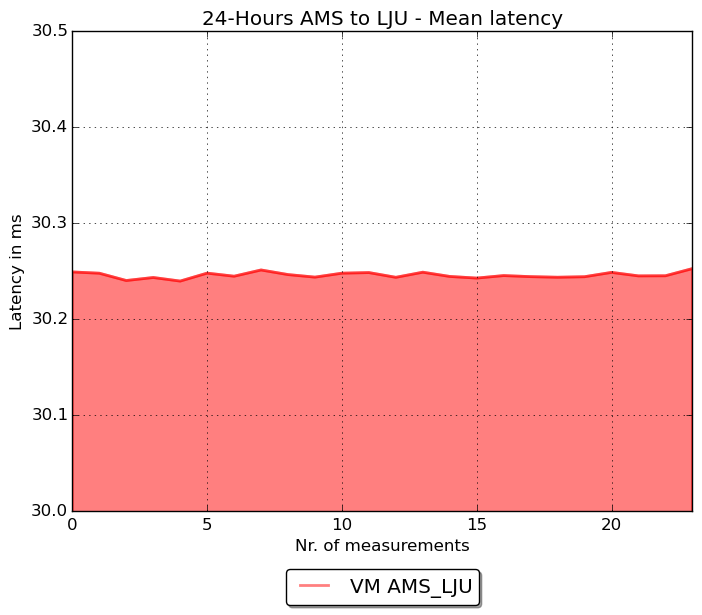
\includegraphics[scale=0.5]{img/24H_AMSLJU_MEANLAT.PNG}
  \caption{Mean Latency on all AMS to LJU circuits}
  \label{fig:sub5}
\end{figure}

\begin{figure}[H]
\centering
  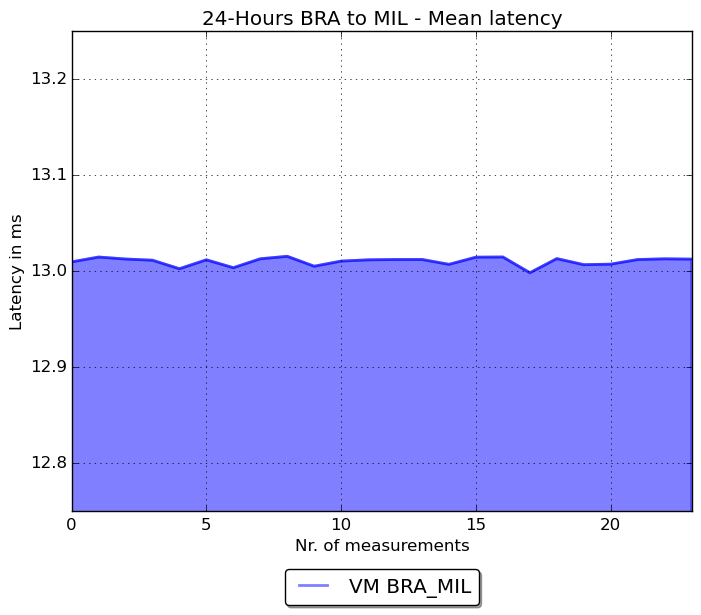
\includegraphics[scale=0.5]{img/24H_BRAMIL_MEANLAT.PNG}
  \caption{Mean Latency on all BRA to MIL circuits}
  \label{fig:sub6}
\end{figure}


\newpage
\section{ Point-to-Point Latency Measurements} \label{app:PtP}
% Please add the following required packages to your document preamble:
% \usepackage{booktabs}
% \usepackage{graphicx}

\setlength\LTleft{0pt}
\setlength\LTright{0pt}
\begin{longtable}{@{\extracolsep{\fill}}lllcccc@{}}
\toprule
\textbf{Instance} & \multicolumn{1}{l}{\textbf{Circuit}} & {\color[HTML]{333333} \textbf{Platform}} & \multicolumn{4}{c}{\textbf{In Milliseconds (ms)}} \\
\textbf{} & \textbf{} & {\color[HTML]{333333} \textbf{}} & \textit{\textbf{Min.}} & \textit{\textbf{Mean}} & \textit{\textbf{99th \%}} & \textit{\textbf{Stddev}} \\ \midrule
\textbf{Libnetwork} & \textit{AMS – MIL} & {\color[HTML]{333333} VM} & 36.3 & 36.5 & 37.0 & 0.1 \\
 &  & {\color[HTML]{333333} Docker} & 36.3 & 36.5 & 37.0 & 0.1 \\ \cmidrule(l){3-7} 
 &  & {\color[HTML]{333333} \textbf{Difference}} & 0.0 & 0.0 & 0.0 & 0.0 \\ \cmidrule(l){2-7} 
 & \textit{AMS – LJU} & {\color[HTML]{333333} VM} & 30.1 & 30.3 & 31.0 & 0.1 \\
 &  & {\color[HTML]{333333} Docker} & 30.1 & 30.3 & 31.0 & 0.1 \\ \cmidrule(l){3-7} 
 &  & {\color[HTML]{333333} \textbf{Difference}} & {\color[HTML]{CB0000} -0.1} & {\color[HTML]{CB0000} -0.1} & 0.0 & 0.0 \\ \cmidrule(l){2-7} 
 & \textit{AMS – BRA} & {\color[HTML]{333333} VM} & 17.5 & 17.7 & 18.0 & 0.1 \\
 &  & {\color[HTML]{333333} Docker} & 17.6 & 17.7 & 18.0 & 0.0 \\ \cmidrule(l){3-7} 
 &  & {\color[HTML]{333333} \textbf{Difference}} & {\color[HTML]{CB0000} -0.1} & {\color[HTML]{CB0000} -0.1} & 0.0 & 0.0 \\ \cmidrule(l){2-7} 
 & \textit{MIL – LJU} & {\color[HTML]{333333} VM} & 61.6 & 62.1 & 62.4 & 0.1 \\
 &  & {\color[HTML]{333333} Docker} & 61.8 & 62.1 & 62.4 & 0.1 \\ \cmidrule(l){3-7} 
 &  & {\color[HTML]{333333} \textbf{Difference}} & {\color[HTML]{CB0000} -0.2} & 0.0 & 0.0 & 0.0 \\ \cmidrule(l){2-7} 
 & \textit{MIL – BRA} & {\color[HTML]{333333} VM} & 12.7 & 13.0 & 14.0 & 0.1 \\
 &  & {\color[HTML]{333333} Docker} & 12.7 & 13.1 & 14.0 & 0.0 \\ \cmidrule(l){3-7} 
 &  & {\color[HTML]{333333} \textbf{Difference}} & 0.0 & {\color[HTML]{CB0000} -0.1} & 0.0 & 0.0 \\ \cmidrule(l){2-7} 
 & \textit{BRA – LJU} & {\color[HTML]{333333} VM} & 47.1 & 47.4 & 48.0 & 0.0 \\
 &  & {\color[HTML]{333333} Docker} & 47.2 & 47.4 & 48.0 & 0.0 \\ \cmidrule(l){3-7} 
 &  & {\color[HTML]{333333} \textbf{Difference}} & 0.0 & {\color[HTML]{CB0000} -0.1} & 0.0 & 0.0 \\ \midrule
\textbf{Weave} & \textit{AMS – MIL} & {\color[HTML]{333333} VM} & 36.1 & 36.4 & 37.0 & 0.0 \\
 &  & {\color[HTML]{333333} Docker} & 36.2 & 36.5 & 37.0 & 0.0 \\ \cmidrule(l){3-7} 
 &  & {\color[HTML]{333333} \textbf{Difference}} & {\color[HTML]{CB0000} -0.1} & {\color[HTML]{CB0000} -0.1} & 0.0 & 0.0 \\ \cmidrule(l){2-7} 
 & \textit{AMS – LJU} & {\color[HTML]{333333} VM} & 29.9 & 30.2 & 31.0 & 0.0 \\
 &  & {\color[HTML]{333333} Docker} & 29.8 & 30.3 & 31.0 & 0.0 \\ \cmidrule(l){3-7} 
 &  & {\color[HTML]{333333} \textbf{Difference}} & 0.0 & {\color[HTML]{CB0000} -0.1} & 0.0 & 0.0 \\ \cmidrule(l){2-7} 
 & \textit{AMS – BRA} & {\color[HTML]{333333} VM} & 17.4 & 17.7 & 18.0 & 0.1 \\
 & \textit{} & {\color[HTML]{333333} Docker} & 17.4 & 17.7 & 18.0 & 0.1 \\ \cmidrule(l){3-7} 
 & \textit{} & {\color[HTML]{333333} \textbf{Difference}} & {\color[HTML]{CB0000} -0.1} & 0.0 & 0.0 & 0.0 \\ \cmidrule(l){2-7} 
 & \textit{MIL – LJU} & {\color[HTML]{333333} VM} & 59.6 & 59.8 & 60.0 & 0.1 \\
 & \textit{} & {\color[HTML]{333333} Docker} & 59.6 & 59.8 & 60.0 & 0.1 \\ \cmidrule(l){3-7} 
 & \textit{} & {\color[HTML]{333333} \textbf{Difference}} & 0.0 & {\color[HTML]{CB0000} -0.1} & 0.0 & 0.0 \\ \cmidrule(l){2-7} 
 & \textit{MIL – BRA} & {\color[HTML]{333333} VM} & 12.8 & 13.0 & 14.0 & 0.1 \\
 &  & {\color[HTML]{333333} Docker} & 12.9 & 13.1 & 14.0 & 0.1 \\ \cmidrule(l){3-7} 
 &  & {\color[HTML]{333333} \textbf{Difference}} & {\color[HTML]{CB0000} -0.1} & {\color[HTML]{CB0000} -0.1} & 0.0 & 0.0 \\ \cmidrule(l){2-7} 
 & \textit{BRA – LJU} & {\color[HTML]{333333} VM} & 43.0 & 43.3 & 44.0 & 0.1 \\
 & \textit{} & {\color[HTML]{333333} Docker} & 43.1 & 59.5 & 130.0 & 0.1 \\ \cmidrule(l){3-7} 
 & \textit{} & {\color[HTML]{333333} \textbf{Difference}} & {\color[HTML]{CB0000} -0.2} & {\color[HTML]{CB0000} -16.2} & {\color[HTML]{CB0000} -86.0} & 0.0 \\ \midrule
\textbf{Flannel} & \textit{AMS – MIL} & {\color[HTML]{333333} VM} & 42.4 & 42.8 & 43.0 & 0.0 \\
 & \textit{} & {\color[HTML]{333333} Docker} & 42.5 & 42.9 & 43.0 & 0.0 \\ \cmidrule(l){3-7} 
 & \textit{} & {\color[HTML]{333333} \textbf{Difference}} & {\color[HTML]{CB0000} -0.1} & {\color[HTML]{CB0000} -0.1} & 0.0 & 0.0 \\ \cmidrule(l){2-7} 
 & \textit{AMS – LJU} & {\color[HTML]{333333} VM} & 29.8 & 30.2 & 31.0 & 0.0 \\
 & \textit{} & {\color[HTML]{333333} Docker} & 29.8 & 30.3 & 31.0 & 0.0 \\ \cmidrule(l){3-7} 
 & \textit{} & {\color[HTML]{333333} \textbf{Difference}} & 0.1 & {\color[HTML]{CB0000} -0.1} & 0.0 & 0.0 \\ \cmidrule(l){2-7} 
 & \textit{AMS – BRA} & {\color[HTML]{333333} VM} & 17.3 & 17.7 & 18.0 & 0.0 \\
 & \textit{} & {\color[HTML]{333333} Docker} & 17.4 & 17.7 & 18.0 & 0.0 \\ \cmidrule(l){3-7} 
 &  & {\color[HTML]{333333} \textbf{Difference}} & {\color[HTML]{CB0000} -0.1} & 0.0 & 0.0 & 0.0 \\ \cmidrule(l){2-7} 
 & \textit{MIL – LJU} & {\color[HTML]{333333} VM} & 55.5 & 55.8 & 56.0 & 0.0 \\
 & \textit{} & {\color[HTML]{333333} Docker} & 55.6 & 55.8 & 56.0 & 0.0 \\
 & \textit{} & {\color[HTML]{333333} \textbf{Difference}} & {\color[HTML]{CB0000} -0.1} & {\color[HTML]{CB0000} -0.1} & 0.0 & 0.0 \\ \cmidrule(l){2-7} 
 & \textit{MIL – BRA} & {\color[HTML]{333333} VM} & 12.8 & 13.0 & 14.0 & 0.0 \\
 & \textit{} & {\color[HTML]{333333} Docker} & 12.9 & 13.1 & 14.0 & 0.0 \\ \cmidrule(l){3-7} 
 & \textit{} & {\color[HTML]{333333} \textbf{Difference}} & {\color[HTML]{CB0000} -0.1} & {\color[HTML]{CB0000} -0.1} & 0.0 & 0.0 \\ \cmidrule(l){2-7} 
 & \textit{BRA – LJU} & {\color[HTML]{333333} VM} & 43.1 & 43.4 & 44.0 & 0.0 \\
 &  & {\color[HTML]{333333} Docker} & 43.1 & 43.4 & 44.0 & 0.0 \\ \cmidrule(l){3-7} 
 &  & {\color[HTML]{333333} \textbf{Difference}} & {\color[HTML]{CB0000} -0.1} & 0.0 & 0.0 & 0.0 \\ \bottomrule
\end{longtable}

\newpage
\section{ Point-to-Point Throughput Measurements} \label{app:PtP_through}

\setlength\LTleft{0pt}
\setlength\LTright{0pt}
\begin{longtable}{@{\extracolsep{\fill}}lclcc@{}}
\toprule
\textbf{Instance} & \multicolumn{1}{l}{\textbf{Circuit}} & {\color[HTML]{333333} \textbf{Platform}} & \multicolumn{2}{l}{\textbf{Throughput in Mbps}} \\
\textbf{} & \textbf{} & {\color[HTML]{333333} \textbf{}} & \textit{\textbf{TCP}} & \textit{\textbf{UDP}} \\ \midrule
\textbf{Libnetwork} & \textit{AMS – MIL} & {\color[HTML]{333333} VM} & 150.7 & 231.6 \\
 &  & {\color[HTML]{333333} Docker} & 213.2 & 110.6 \\ \cmidrule(l){3-5} 
 &  & {\color[HTML]{333333} \textbf{Difference}} & {\color[HTML]{CB0000} -62.5} & {\color[HTML]{009901} 121.1} \\ \cmidrule(l){2-5} 
 & \textit{AMS – LJU} & {\color[HTML]{333333} VM} & 152.5 & 223.3 \\
 &  & {\color[HTML]{333333} Docker} & 165.3 & 110.0 \\ \cmidrule(l){3-5} 
 &  & {\color[HTML]{333333} \textbf{Difference}} & {\color[HTML]{CB0000} -12.8} & {\color[HTML]{009901} 113.3} \\ \cmidrule(l){2-5} 
 & \textit{AMS – BRA} & {\color[HTML]{333333} VM} & 148.9 & 225.5 \\
 &  & {\color[HTML]{333333} Docker} & 207.1 & 109.9 \\ \cmidrule(l){3-5} 
 &  & {\color[HTML]{333333} \textbf{Difference}} & {\color[HTML]{CB0000} -58.2} & {\color[HTML]{009901} 115.6} \\ \cmidrule(l){2-5} 
 & \textit{MIL – LJU} & {\color[HTML]{333333} VM} & 127.4 & 238.4 \\
 &  & {\color[HTML]{333333} Docker} & 128.3 & 130.1 \\ \cmidrule(l){3-5} 
 &  & {\color[HTML]{333333} \textbf{Difference}} & {\color[HTML]{CB0000} -0.8} & {\color[HTML]{009901} 108.3} \\ \cmidrule(l){2-5} 
 & \textit{MIL – BRA} & {\color[HTML]{333333} VM} & 181.2 & 254.5 \\
 &  & {\color[HTML]{333333} Docker} & 167.0 & 129.2 \\ \cmidrule(l){3-5} 
 &  & {\color[HTML]{333333} \textbf{Difference}} & {\color[HTML]{009901} 14.2} & {\color[HTML]{009901} 125.4} \\ \cmidrule(l){2-5} 
 & \textit{BRA – LJU} & {\color[HTML]{333333} VM} & 158.8 & 226.7 \\
 &  & {\color[HTML]{333333} Docker} & 133.7 & 111.8 \\ \cmidrule(l){3-5} 
 &  & {\color[HTML]{333333} \textbf{Difference}} & {\color[HTML]{009901} 25.0} & {\color[HTML]{009901} 114.8} \\ \midrule
\textbf{Weave} & \textit{AMS – MIL} & {\color[HTML]{333333} VM} & 179.0 & 272.8 \\
 &  & {\color[HTML]{333333} Docker} & 243.0 & 130.5 \\ \cmidrule(l){3-5} 
 &  & {\color[HTML]{333333} \textbf{Difference}} & {\color[HTML]{CB0000} -64.0} & {\color[HTML]{009901} 142.2} \\ \cmidrule(l){2-5} 
 & \textit{AMS – LJU} & {\color[HTML]{333333} VM} & 189.2 & 249.9 \\
 &  & {\color[HTML]{333333} Docker} & 201.6 & 129.3 \\ \cmidrule(l){3-5} 
 &  & {\color[HTML]{333333} \textbf{Difference}} & {\color[HTML]{CB0000} -12.4} & {\color[HTML]{009901} 120.6} \\ \cmidrule(l){2-5} 
 & \textit{AMS – BRA} & {\color[HTML]{333333} VM} & 188.5 & 255.4 \\
 & \textit{} & {\color[HTML]{333333} Docker} & 209.8 & 128.9 \\ \cmidrule(l){3-5} 
 & \textit{} & {\color[HTML]{333333} \textbf{Difference}} & {\color[HTML]{CB0000} -21.2} & {\color[HTML]{009901} 126.5} \\ \cmidrule(l){2-5} 
 & \textit{MIL – LJU} & {\color[HTML]{333333} VM} & 131.7 & 255.3 \\
 & \textit{} & {\color[HTML]{333333} Docker} & 161.5 & 128.5 \\ \cmidrule(l){3-5} 
 & \textit{} & {\color[HTML]{333333} \textbf{Difference}} & {\color[HTML]{9A0000} -29.8} & {\color[HTML]{009901} 126.8} \\ \cmidrule(l){2-5} 
 & \textit{MIL – BRA} & {\color[HTML]{333333} VM} & 188.5 & 261.0 \\
 &  & {\color[HTML]{333333} Docker} & 217.9 & 130.4 \\ \cmidrule(l){3-5} 
 &  & {\color[HTML]{333333} \textbf{Difference}} & {\color[HTML]{CB0000} -29.3} & {\color[HTML]{009901} 130.6} \\ \cmidrule(l){2-5} 
 & \textit{BRA – LJU} & {\color[HTML]{333333} VM} & 149.9 & 229.0 \\
 & \textit{} & {\color[HTML]{333333} Docker} & 43.9 & 17.2 \\ \cmidrule(l){3-5} 
 & \textit{} & {\color[HTML]{333333} \textbf{Difference}} & {\color[HTML]{009901} 106.0} & {\color[HTML]{009901} 211.8} \\ \midrule
\textbf{Flannel} & \textit{AMS – MIL} & {\color[HTML]{333333} VM} & 177.1 & 271.9 \\
 & \textit{} & {\color[HTML]{333333} Docker} & 187.5 & 126.9 \\ \cmidrule(l){3-5} 
 & \textit{} & {\color[HTML]{333333} \textbf{Difference}} & {\color[HTML]{CB0000} -10.4} & {\color[HTML]{009901} 145.0} \\ \cmidrule(l){2-5} 
 & \textit{AMS – LJU} & {\color[HTML]{333333} VM} & 180.2 & 268.1 \\
 & \textit{} & {\color[HTML]{333333} Docker} & 225.6 & 128.3 \\ \cmidrule(l){3-5} 
 & \textit{} & {\color[HTML]{333333} \textbf{Difference}} & {\color[HTML]{CB0000} -45.4} & {\color[HTML]{009901} 139.8} \\ \cmidrule(l){2-5} 
 & \textit{AMS – BRA} & {\color[HTML]{333333} VM} & 187.2 & 267.0 \\
 & \textit{} & {\color[HTML]{333333} Docker} & 169.8 & 127.8 \\ \cmidrule(l){3-5} 
 &  & {\color[HTML]{333333} \textbf{Difference}} & {\color[HTML]{009901} 17.4} & {\color[HTML]{009901} 139.2} \\ \cmidrule(l){2-5} 
 & \textit{MIL – LJU} & {\color[HTML]{333333} VM} & 142.2 & 278.8 \\
 & \textit{} & {\color[HTML]{333333} Docker} & 210.7 & 131.9 \\
 & \textit{} & {\color[HTML]{333333} \textbf{Difference}} & {\color[HTML]{CB0000} -68.6} & {\color[HTML]{009901} 146.9} \\ \cmidrule(l){2-5} 
 & \textit{MIL – BRA} & {\color[HTML]{333333} VM} & 194.2 & 254.0 \\
 & \textit{} & {\color[HTML]{333333} Docker} & 211.3 & 130.6 \\ \cmidrule(l){3-5} 
 & \textit{} & {\color[HTML]{333333} \textbf{Difference}} & {\color[HTML]{CB0000} -17.1} & {\color[HTML]{009901} 123.4} \\ \cmidrule(l){2-5} 
 & \textit{BRA – LJU} & {\color[HTML]{333333} VM} & 151.7 & 243.2 \\
 &  & {\color[HTML]{333333} Docker} & 214.6 & 110.0 \\ \cmidrule(l){3-5} 
 &  & {\color[HTML]{333333} \textbf{Difference}} & {\color[HTML]{CB0000} -63.0} & {\color[HTML]{333333} 133.2} \\ \bottomrule
\end{longtable}

\newpage
\section{ Streaming media measurements} \label{app:stream}
\begin{table}[!ht]
\small
\centering
\resizebox{\textwidth}{!}{%
\begin{tabular}{@{}lcccccc@{}}
\toprule
\multicolumn{1}{c}{} & \textbf{Circuit} & \textbf{Workers} & \multicolumn{3}{c}{\textbf{Bit rate (Kbps)}} & \textbf{Jitter (ms)} \\
\rowcolor[HTML]{FFFFFF} 
 & \textbf{} & \textbf{} & \textit{\textbf{Min.}} & \textit{\textbf{Mean}} & \textit{\textbf{Max.}} & \textbf{} \\ \midrule
\textbf{VM} & \textit{BRA – AMS} & 1 & 112.09 & 957.59 & 1853.68 & 0.08 \\ 
\textbf{} & \textit{} & 3 & 69.59 & 681.23 & 1429.48 & 0.45 \\
\textbf{} & \textit{} & 9 & 41.18 & 272.17 & 944.11 & 2.10 \\
\textbf{} & \textit{BRA – MIL} & 1 & 111.19 & 955.46 & 1854.89 & 0.09 \\
\textbf{} & \textit{} & 3 & 69.13 & 671.21 & 1426.39 & 0.55 \\
\textbf{} & \textit{} & 9 & 39.40 & 273.45 & 932.24 & 2.00 \\
\textbf{} & \textit{BRA – LJU} & 1 & 111.33 & 948.15 & 1851.54 & 0.09 \\
\textbf{} & \textit{} & 3 & 68.99 & 670.25 & 1421.54 & 0.49 \\
\textbf{} & \textit{} & 9 & 40.49 & 268.25 & 919.55 & 1.92 \\ \midrule
\textbf{Weave} & \textit{BRA – AMS} & 1 & 113.20 & 958.70 & 1851.37 & 0.10 \\
\textbf{} & \textit{} & 3 & 68.93 & 654.39 & 1422.14 & 0.47 \\
\textbf{} & \textit{} & 9 & 40.17 & 270.41 & 941.41 & 2.14 \\
\textbf{} & \textit{BRA – MIL} & 1 & 108.47 & 948.94 & 1849.74 & 0.09 \\
\textbf{} & \textit{} & 3 & 70.52 & 648.69 & 1409.49 & 0.49 \\
\textbf{} & \textit{} & 9 & 39.35 & 272.28 & 935.86 & 1.86 \\
\textbf{} & \textit{BRA – LJU} & 1 & 109.74 & 944.86 & 1834.43 & 0.09 \\
\textbf{} &  & 3 & 66.23 & 650.13 & 1414.70 & 0.47 \\
\textbf{} &  & 9 & 41.09 & 269.38 & 928.17 & 2.29 \\ \midrule
\textbf{Libnetwork} & \textit{BRA – AMS} & 1 & 113.79 & 963.13 & 1868.45 & 0.06 \\
\textbf{} & \textit{} & 3 & 67.78 & 659.49 & 1445.72 & 0.46 \\
\textbf{} & \textit{} & 9 & 40.22 & 277.33 & 941.81 & 2.01 \\
\textbf{} & \textit{BRA – MIL} & 1 & 109.93 & 949.45 & 1799.31 & 0.06 \\
\textbf{} & \textit{} & 3 & 69.98 & 650.90 & 1416.16 & 0.48 \\
\textbf{} & \textit{} & 9 & 38.96 & 273.05 & 934.06 & 1.74 \\
\textbf{} & \textit{BRA – LJU} & 1 & 112.00 & 948.27 & 1833.70 & 0.08 \\
\textbf{} & \textit{} & 3 & 72.79 & 642.49 & 1426.46 & 0.50 \\
\textbf{} &  & 9 & 37.44 & 271.10 & 917.75 & 1.98 \\ \midrule
\textbf{Flannel} & \textit{BRA – AMS} & 1 & 109.87 & 947.41 & 1837.20 & 0.11 \\
\textbf{} & \textit{} & 3 & 64.24 & 632.10 & 1402.66 & 0.40 \\
\textbf{} & \textit{} & 9 & 40.33 & 274.38 & 944.66 & 2.28 \\
\textbf{} & \textit{BRA – MIL} & 1 & 105.56 & 947.71 & 1829.12 & 0.13 \\
\textbf{} & \textit{} & 3 & 66.53 & 621.74 & 1427.34 & 0.45 \\
\textbf{} & \textit{} & 9 & 40.10 & 272.09 & 928.99 & 1.91 \\
\textbf{} & \textit{BRA – LJU} & 1 & 110.88 & 946.26 & 1844.49 & 0.10 \\
\textbf{} & \textit{} & 3 & 62.97 & 623.68 & 1467.22 & 0.46 \\
\textbf{} &  & 9 & 41.26 & 267.24 & 916.67 & 2.43 \\ \midrule
\end{tabular}
}
\end{table}
  
\end{appendices}